\documentclass{ximera}
%\addPrintStyle{..}

\begin{document}
	\author{Bart Lambregs}
	\xmtitle{De eerste wet van Newton}{}
    \xmsource\xmuitleg
	
Om een boek met een constante snelheid over de tafel te duwen, is een zekere kracht nodig. Met een smeermiddel tussen boek en tafel is al minder kracht nodig. In de praktijk geen wrijving realiseren is niet mogelijk maar duidelijk is dat hoe minder wrijving hoe minder kracht nodig is om het boek met een constante snelheid te laten bewegen. Eenmaal in beweging gebracht, nadert de benodigde kracht tot nul, en dat terwijl het boek met constante snelheid blijft bewegen.

Door aan te nemen dat er geen kracht nodig is om in beweging te blijven, valt deze opeenvolging van waarnemingen te verklaren.

Deze aanname zit vervat in de eerste wet van Newton.

\begin{definition}
{\textbf{De eerste wet van Newton}}\nl

Een voorwerp behoudt zijn toestand van rust of van eenparige rechtlijnige beweging, tenzij er een resulterende kracht op werkt.
\end{definition}

\begin{remark}{De eerste wet van Newton wordt ook wel de traagheidswet genoemd.}
	De eigenschap dat een lichaam zijn rust of constante snelheid op een rechte lijn behoudt, wordt inertie of traagheid genoemd. Vandaar de alternatieve naam voor de wet.
\end{remark}

\begin{denkvraag*}{}
	Als je tegen een van \SI{300}{km/h} in de Thalys richting Parijs zit, voel je de zetel dan harder tegen jou duwen dan dat ze dat doet wanneer je nog stilstaat in Brussel-Zuid?
\end{denkvraag*}

\begin{denkvraag*}{}
	\begin{enumerate}
		\item Hoe kunnen de broers Staf en Mathias Coppens in het filmpje gemaakt voor het programma Het Lichaam van Coppens blijven bewegen door de lucht terwijl de zetel toch niet meer duwt?
		\item Waarom wrijven de broers bruine zeep op de plank?
	\end{enumerate}

	\begin{center}
		\youtube{l-X8sG1JV6Q}
	\end{center}

\end{denkvraag*}

\begin{exercise}
	Wanneer je met de fiets fietst, rechtdoor en met een constante snelheid, dan is de kracht die je voorwaarts uitoefent 
	%\begin{multipleChoice}
	\wordChoice{
		\choice{groter dan}
		\choice{kleiner dan}
		\choice[correct]{gelijk aan}
	}
	%\end{multipleChoice}
	de weerstandskracht die achterwaarts is gericht? 
	\\
	Met andere woorden: de resulterende kracht op jouw fiets is dan
	\wordChoice{
		\choice{naar voren gericht}
		\choice[correct]{nul}
		\choice{naar achteren gericht}
	}
	.
	\begin{oplossing}
		De resulterende kracht is nul! 
		Want als er een resulterende kracht was, dan zou volgens de wet van de traagheid de toestand van eenparige rechtlijnige beweging niet worden behouden, en zou je ofwel trager ofwel sneller gaan rijden.

		Als je met een constante snelheid fiets, is de kracht die je uitoefent precies voldoende om alle wrijvingskrachten op te heffen. Als je minder kracht uitoefent, vertraag je en als je meer kracht uitoefent versnel je.
	\end{oplossing}
\end{exercise}

\begin{exercise}
	Als je plots remt met je fiets kan je over je stuur vliegen. Hoe komt dat?
	\begin{oplossing}
		Volgens de wet van de traagheid wil je je toestand van beweging voortzetten. Omdat de fiets slechts een beperkte kracht op jou kan uitoefenen, bestaat de kans dat die niet groot genoeg is om je tot stilstand te brengen.
	\end{oplossing}
\end{exercise}

\end{document}



% Op 22 oktober 1895 gebeurde er in het eindstation Gare Montparnasse -- Parijs, een ongeluk. De treinbestuurder was door het station gereden en pas 30 meter voorbij het einde van het spoor tot stilstand gekomen.
% 	\begin{image}
% 	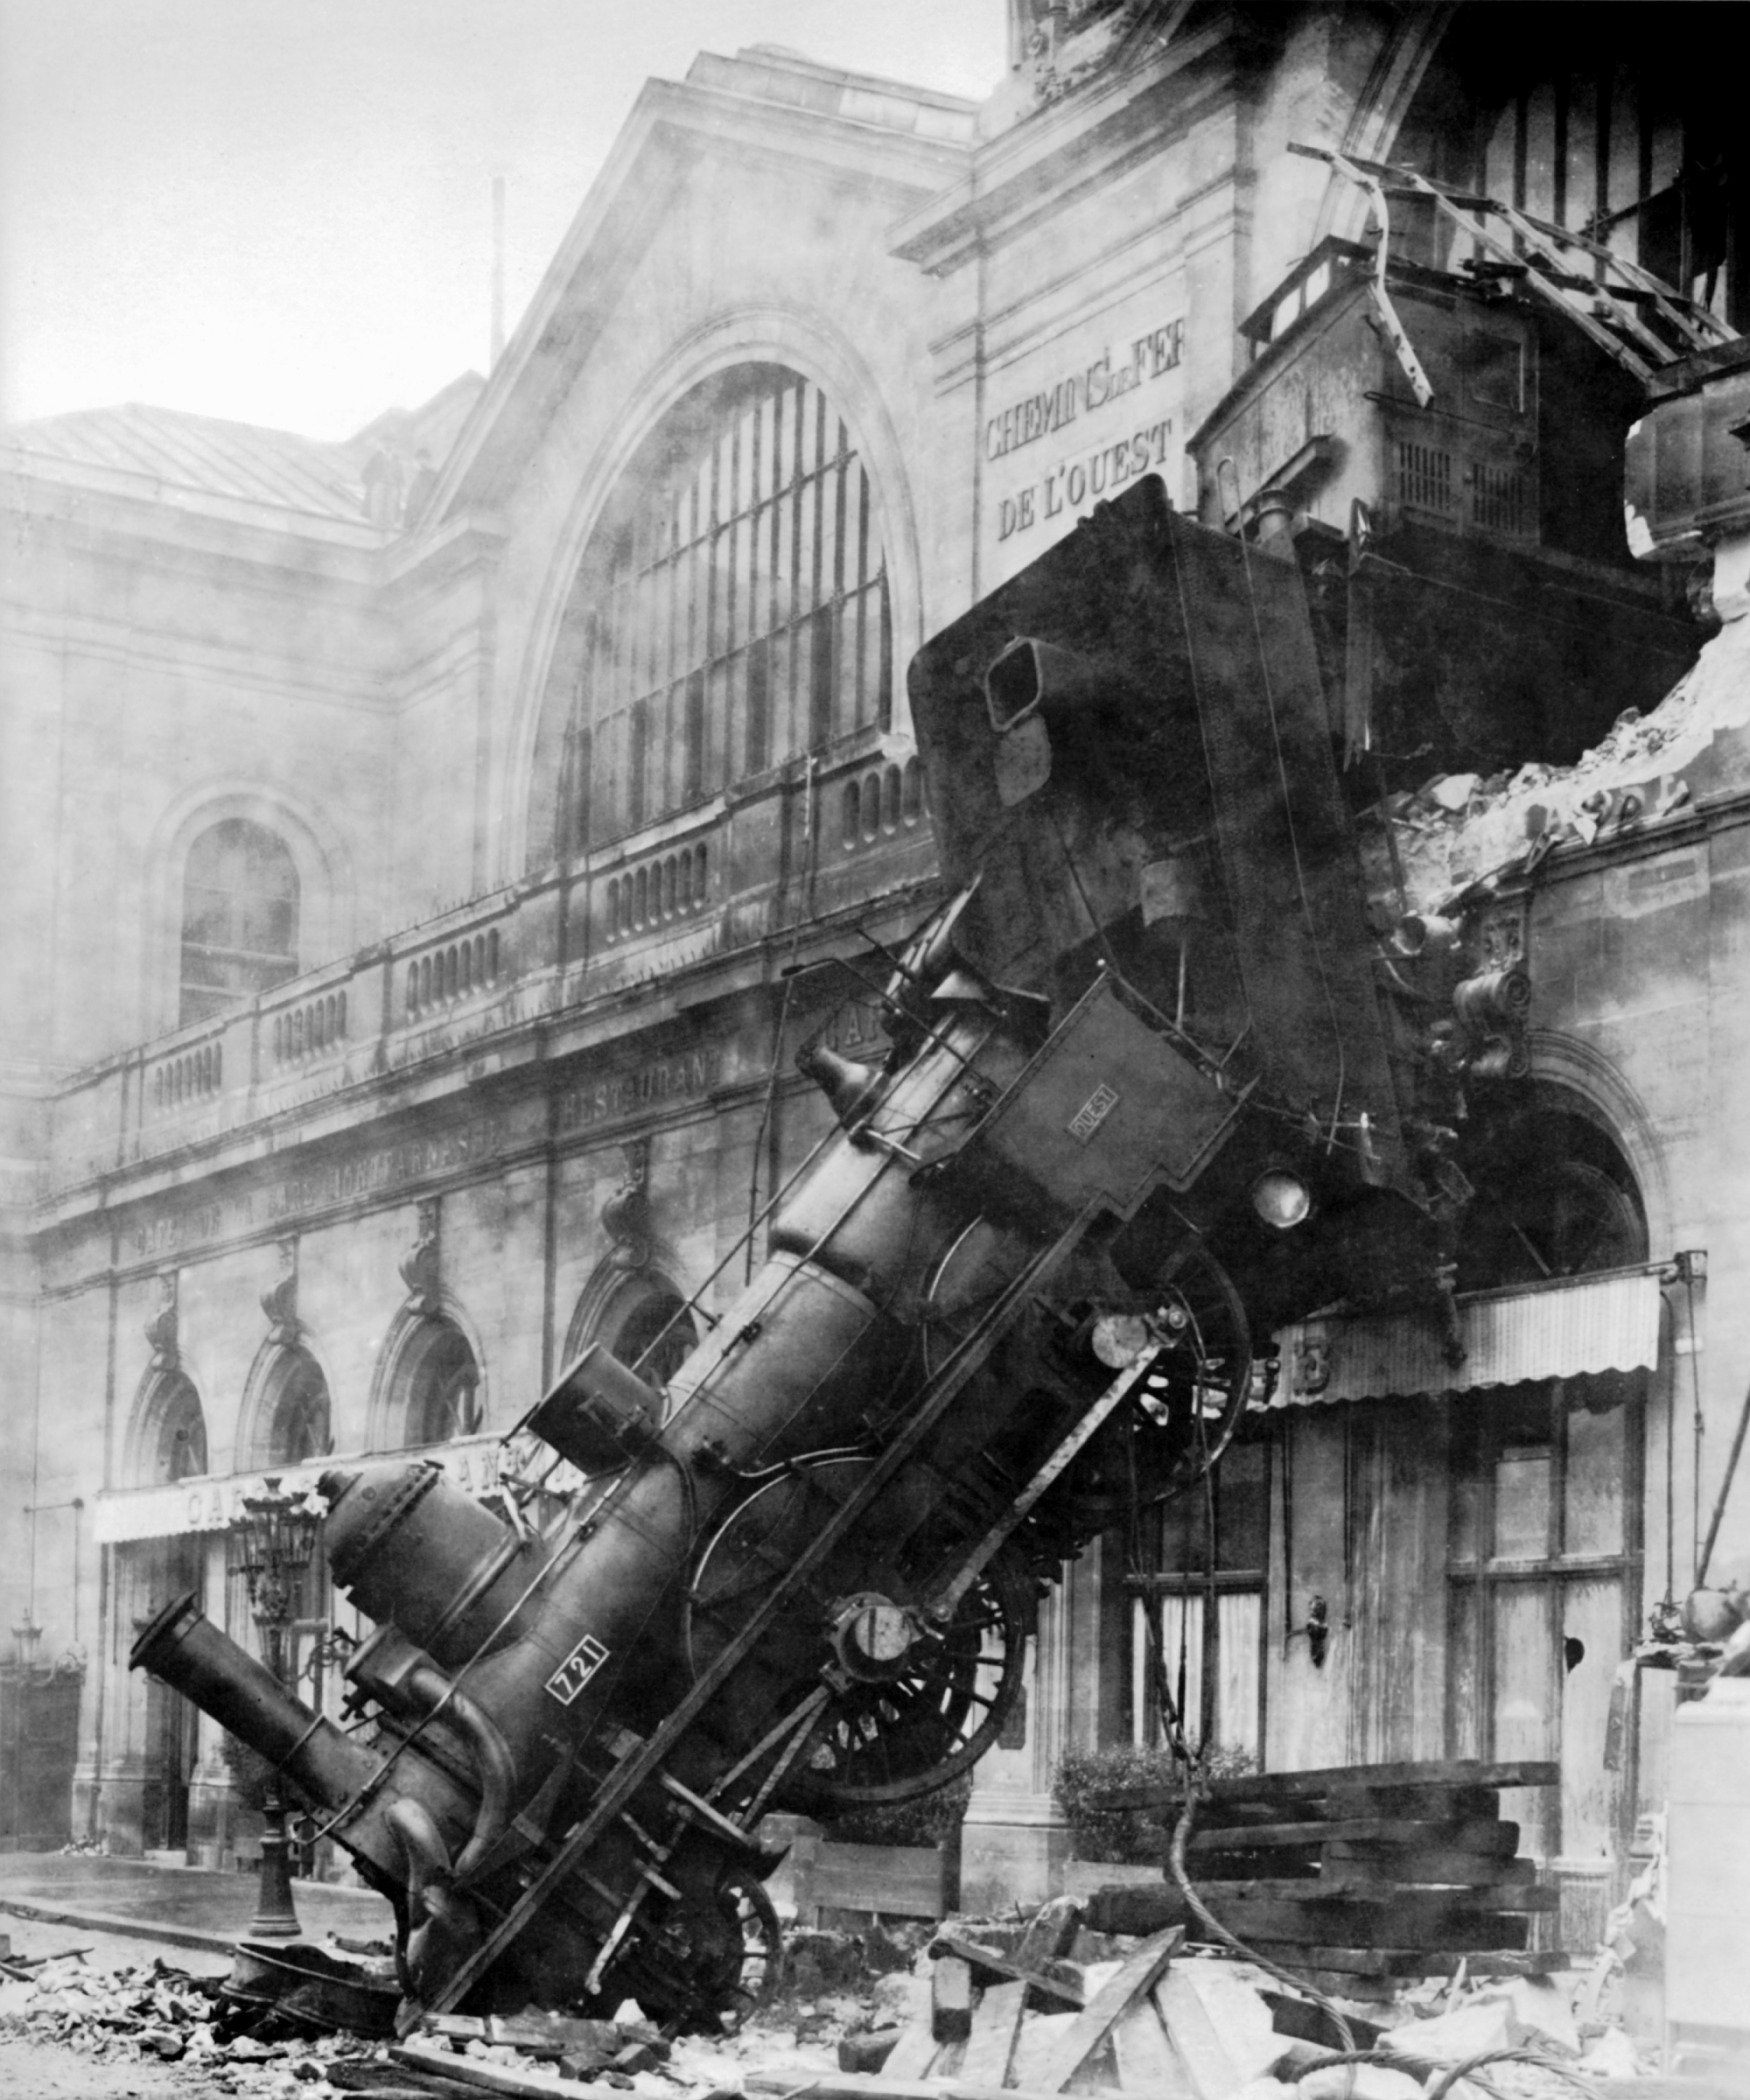
\includegraphics[width=.8\textwidth]{Train_wreck_at_Montparnasse_1895}
% 	\end{image}
% 	\captionof{figure}{Gare Montparnasse. Parijs 1895}
	
% 	De figuur ademt de onvermijdelijke wet van de traagheid uit \ldots